\documentclass[11pt]{article}

\usepackage[T1]{fontenc}
\usepackage[margin=0.8in]{geometry}
\usepackage{amsmath,amssymb}
\usepackage{graphicx}
\usepackage{caption}
\usepackage{titlesec}
\usepackage{hyperref}
\graphicspath{{../../../figures/}}

\captionsetup{font=small,labelfont=bf}
\titleformat{\section}{\normalfont\large\bfseries}{}{0pt}{}
\titlespacing*{\section}{0pt}{8pt}{2pt}
\setlength{\parskip}{4pt}
\setlength{\parindent}{0pt}
\pagestyle{empty}

\begin{document}

\begin{center}
{\Large\bfseries Managing Sea-Level Rise Risk}\\[3pt]
{\normalsize How West Antarctica changes the nature of the problem}
\end{center}

Sea level rises from four main sources: seawater expanding as it warms, melting mountain glaciers, ice loss from Greenland, and ice flowing from Antarctica into the ocean. The first three respond to temperature in ways that are relatively well understood and predictable. More warming produces more sea-level rise, and limiting warming reduces it.

West Antarctica behaves differently. Several of its fastest-changing glaciers, including Thwaites, are retreating over bedrock that lies below sea level and slopes downward inland. As they retreat, more ice can flow toward the ocean, potentially setting off a feedback in which retreat leads to further retreat. Once that process is underway it is driven by the shape of the bed rather than by continued warming, which means reducing temperatures may not be enough to stop it. The observational record is too short to tell us whether it has already begun.

That distinction changes the structure of sea-level risk, and Ar\'{e}te's SPECTRUM forecast is built to show where the structure changes. SPECTRUM models each sea-level contributor separately and tunes each model against decades of observations of that contributor alone. The record of global sea level itself is withheld and used only to test the finished forecast. That test is the point. Driven by observed temperatures, the model closes 97 to 103\% of the rate of rise measured by satellites since 1993 and matches the observed record back to 1950. That window spans about 1.2 $^\circ$C of warming, comparable to the warming over the coming decades, so skill against the past is a reasonable basis for confidence in the SPECTRUM forecast. Because the model never saw the answer it was asked to reproduce, the match is validation rather than a fit.

That validation covers every contributor except West Antarctica, whose record is too short to settle the question. SPECTRUM therefore carries West Antarctica as two explicit futures: one in which ice loss continues along its observed path, and one in which it accelerates. The forecast is not a single range of outcomes. It is two worlds, and we do not yet know which one we are in.

In the first world the problem is the familiar one. Warming drives the rise, and cutting warming cuts the rise. If Thwaites and its neighbors hold, sea level will about 0.66 m between 2000 and 2100 under the warming that current policies imply. The worst case, the level with a 1-in-20 chance of being exceeded, is 0.84 m. Holding warming to 2 rather than 4 $^\circ$C avoids roughly 36 cm of that rise. The range is narrow and emissions policy moves it.

The second world is different in kind. If Thwaites destabilizes, the typical outcome rises only modestly, to about 0.85 m, but the reasonable worst case increases almost a meter, to 1.81 m. That is the shape of the problem. West Antarctica does not so much raise the sea level we expect as open a long, high-risk tail of outcomes. This is why West Antarctica accounts for more than 90\% of the uncertainty in the forecast.

The tail risk is the part emissions cuts cannot close, and the forecast shows it directly. If Thwaites remains stable, deep emissions cuts nearly halve the worst case, from 1.11 m at 4 $^\circ$C to 0.62 m at 2 $^\circ$C. If Thwaites is unstable, the same cuts move the worst case only from 2.01 m to 1.62 m, and it stays near 2 m whatever the world does about emissions. This is the physical point made concrete: a retreat that feeds on the shape of the bed beneath the ice does not respond to the thermostat. Emissions largely determine how much sea-level rise is likely. West Antarctica determines how severe it could become.

This is not an abstract distinction. Coastal planners build to the reasonable worst case, and the gap between the two worlds moves that level by nearly a meter. That gap puts on the order of 180 million additional people below the annual flood line, adds roughly US\$130 billion per year in coastal adaptation costs, and adds trillions of dollars per year in flood damages wherever adaptation does not keep pace. Much of that choice has to be made long before 2100, because coastal infrastructure lasts for decades.

\begin{figure}[t!]
\centering
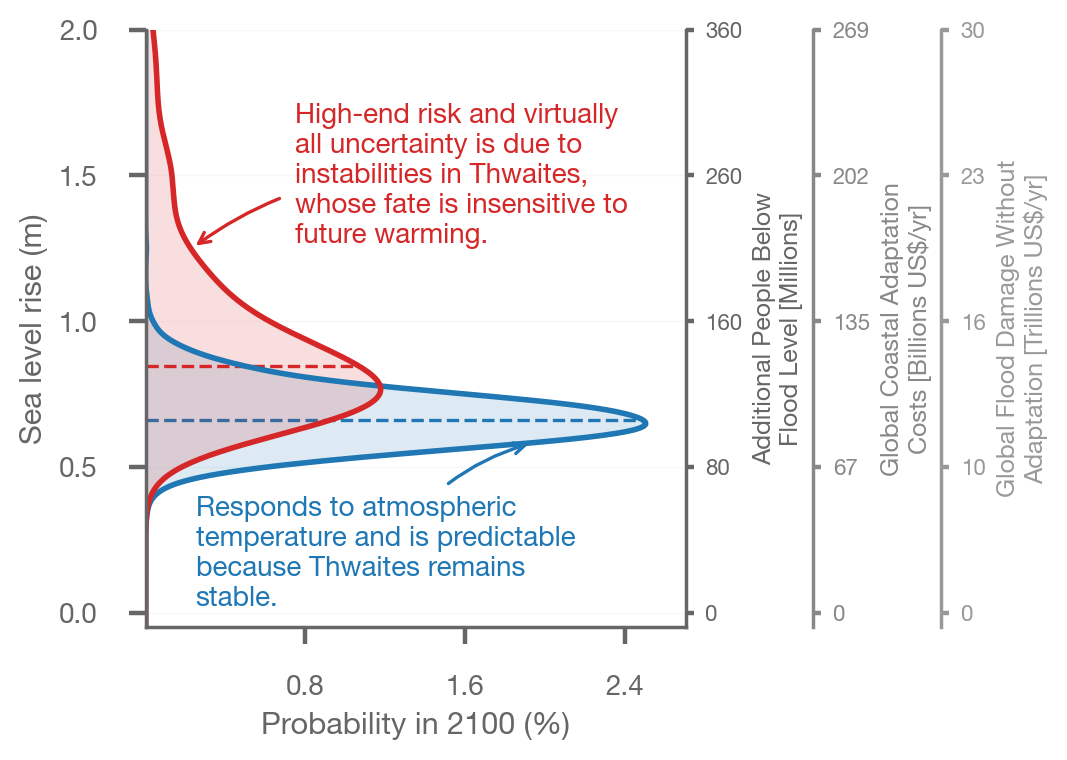
\includegraphics[width=0.68\textwidth]{wais_probability2100_simple.png}
\caption{Two worlds. The chance of each level of global sea-level rise by 2100, relative to the year 2000, under the warming that current policies imply. The blue curve is the forecast if Thwaites Glacier remains stable, and the red curve is the forecast if it does not. Dashed lines mark the typical outcome of each. The medians differ by less than 0.2 m; what matters is the long red tail, which emissions cuts do not remove. Right-hand scales convert rise into people below flood level, annual adaptation costs, and annual flood damages without adaptation.}
\label{fig:forecast}
\end{figure}

\section{Managing this risk requires two different strategies}

The first is familiar. Cutting emissions and removing carbon from the atmosphere reduce thermal expansion and ice loss from the temperature-responsive parts of the system. These actions remain essential and avoid tens of centimeters of rise.

The second is to find out which world we are in, and whether we can change it. We do not know today whether rapid retreat is underway, how quickly it could unfold, or whether it could be slowed. Answering those questions requires substantially better observations of West Antarctica, sustained long enough to matter, and research into the physical processes that govern these glaciers. The single most informative measurement is the rate of West Antarctic ice loss over the coming two decades.

That knowledge has a price, and we can estimate it. Resolving whether West Antarctic loss will be slow or rapid is worth on the order of \$5 trillion in avoided adaptation costs, and the value falls the later the answer arrives, because late answers leave fewer decisions left to improve. Even a partial answer, well short of certainty, would justify research spending far above current levels. Learning more is not the same as being reassured. It is as likely as not that further research strengthens the case for rapid loss; the value lies in resolving the question, not in the answer being favorable.

It also warrants careful investigation of whether additional tools could eventually reduce the risk itself. In the forecast's own terms, stabilizing West Antarctica means making the slow world more likely and the fast world less severe, a target any proposed intervention can be measured against. Whether any intervention could safely and effectively slow that loss remains an open question, alongside significant questions about side effects and governance. The immediate task is not deployment. It is to understand the risk, establish which approaches are physically plausible, and learn what options the world may have if West Antarctic loss accelerates.

Reducing warming remains essential. So does understanding whether the risks posed by West Antarctic ice loss can be reduced.


\end{document}
